\chapter{Research}

 In the projects research stage, different technologies and tools as well as some development techniques will be discussed.
%%%%%%%%%%%%%%%%%%%%%%%%%%%%%%%%%%%%%
%%%%%     METHODOLOGY'S         %%%%%
%%%%%%%%%%%%%%%%%%%%%%%%%%%%%%%%%%%%%
 \section{Methodologies}
  Methodologies are describing the method a project should be handled. They mostly define several stages or phases in which the developer had to complete a few tasks. Each methodology has its own ways to handle tasks like analysis, design, implementation and testing. If a project follows a specific methodology then the developers as well as the project manager should always know in which state the project is and how long it will take to reach a previously defined point. Some methodologies also have a detailed description how the customer should be included in the development process.

  This project needs a methodology because the developer should always know what the current status of the project is and how much work is still left. This project has a defined beginning and a defined end, therefore the planing and designing can be made for the whole project, right before the coding will start.
  \label{sec:research:methodology}
  \subsection{Waterfall life cycle}
   The knowledge for this methodology came from the following two books, \citet[p.73--77]{FabrizioFioravanti:2005} and \citet[p.138--140]{HRHansen:1998}.

   In the waterfall methodology all defining work has to be done before the coding can be started. Therefore all use cases and functionalities have to be described right before the implementation will start. This is why the project will be divided into single stages, each stage then will be done after its predecessor. So entering the next phase of a project is only possible if the one before is already completed. The five main stages of the waterfall methodology are (in this order): feasibility study, analysis, project specification, development, integration and testing, deployment and maintenance. In the following these phases will be described in detail.

   \subsubsection*{Feasibility study}
    In this stage the feasibility of the project is checked: is it affordable, technically manageable and legal.

   \subsubsection*{Analysis}
    In this stage of the project the functional details needed to be analysed and written down. The outcome of the stage are several documents that will describe the system and its surroundings in detail. Following is a detailed description affords a:
    \begin{itemize}
     \item Requirement specification document (RSD), describes the application and all its use cases, explained in all their detail. This document includes information regarding the user interfaces, as long as there are such interfaces. It will also show the workflow of the application.
     \item System test plan (STP), this document includes a full strategy about testing the application. All the possible test cases should be written down, as well as their expected outcome.
    \end{itemize}

   \subsubsection*{Project specification}
    In this phase the project manager will do the most work. He needs to define the software architecture and the technologies of this project. Therefore he will use the RSD to create those specifications adequate to each defined task of the application. This last aspect of this stage is to verify the milestones and the time line of the whole project. The project specification document (PSD) will be the outcome of this phase. This document includes all previously analysed data and all aspects of the architecture in detail.

   \subsubsection*{Development}
    This stage is the main stage of the project. The project manager has to keep track of the project and has to look at the current stage of the project and if there will be problems that will cause a noncompliance to the planned time schedule. The developers on the other hand have to program and document the code. The outcome of this stage will be the source code and a code description.

   \subsubsection*{Integration and testing}
    This phase is split into two parts. The first part is the integration of all modules to one project, if necessary the developers need to reprogram the relevant parts. After everything fits together the second part will be the testing of the whole project. Depending on the developed project, this part needs to be a testing environment or not. The test phase normally is divided into two subparts, the alpha and the beta phase. Whilst in the alpha phase everything is tested in a closed environment and with a special look if everything is working like it is described in the STP (see Analysis), the beta phase includes costumers to test the product in their environment.

   \subsubsection*{Deployment}
    At the deployment phase the project will be installed in the customers environment. All the debug and logging features that were necessary for the testing phase are switched off or taken from the code. Usually the end of the beta, start of the maintenance and start of the deployment phase are at the same time

   \subsubsection*{Maintenance}
    In the maintenance phase the errors detected during the test phase will be corrected and delivered to the customer.

   \subsubsection*{Pros and cons}
    \begin{itemize}
     \item \textbf{Pro}
      \begin{itemize}
       \item Usable for small teams.
       \item Good if the project has a fixed finishing date
      \end{itemize}
     \item \textbf{Con}
      \begin{itemize}
       \item Not very flexible, if something went wrong during the research stage it will break the methodology if it will be found at the implementation stage.
       \item Not usable for projects that will be improved during the development process.
      \end{itemize}
    \end{itemize}

  \subsection{Rapid application development (RAD)}
   The Rapid application development (RAD) uses the waterfall idea for its internal phases. Instead of waiting that every phase ends, RAD is focused to create a prototype real fast. The prototype is split into different phases, analysis, design and prototyping. After the prototype is done it will be shown to the users of the system. Then the users have the ability to ask for changes and improvements. After this the whole prototyping phase starts over again, the changes and improvements of the users get involved into the new analysis, design and prototyping phase. Then the new prototype will again be brought to the users. This will loop as long as the users have something left to improve or the project manager will call a stop to the project.

   The vantages of this system are that the users are included into the development process and their wishes are included directly on the development. The user can identify himself with the product and acquires the functions it provides faster.

   One of the disadvantages is that the project has no defined end, if the users are asking for more and more features then it will not have an end. In that case the project manager has to stop the prototyping phases before the project runs out of money. Another disadvantage is that the user might have the feeling that the project is nearly done after the last prototype. But the prototype is still a prototype, a program that is put together fast with no thought out design of the full system, no user documentation and mostly no source documentation
   \citep[p.25--28]{HentzenWhil:2002}
   \subsubsection*{Pros and cons}
    \begin{itemize}
     \item \textbf{Pro}
      \begin{itemize}
       \item Good for projects with no fixed end.
       \item Good for larger teams.
       \item Good for projects where the specification may change during development.
       \item Good for the customer to see that there is progress during the development.
       \item User is directly included into the development process.
      \end{itemize}
     \item \textbf{Con}
      \begin{itemize}
       \item Bad for projects with fixed end.
       \item Bad if the customer want to have more and more features after every cycle.
       \item Bad because the application shown is a prototype only and the customer may think that it is a full, nearly done application.
       \item Not usable for non customer orientated projects.
      \end{itemize}
    \end{itemize}

  \subsection{Extreme Programming (XP)}
   The following methodology is written out of the knowledge from the following resources, \citet{wikipedia:ExtremeProgramming} and the following resources to verify the information provided by Wikipedia. First of all the book and web page by the inventor of extreme programming \citet{KentBeck:2005} and \citet{KentBeck:ExtremeProgramming}, as well as the books by \citet[p.108--132]{FabrizioFioravanti:2005} and by \citet[p.1--9]{RichardHightower:2004}.

   Extreme Programming is based on the RAD methodology but adds a some more rules regarding the surroundings and the treatment of the customers. The whole methodology is based on the following five values and a bunch of principles and practices. But as Kent himself is saying theses rules are bendable and some might be dropped in certain circumstances and therefore other rules might come up. Those rules are depending on the company and the product the company is producing, if for example the project is a project which might risk human lives it should be possible, in any state of the project, to follow the whole chain of development back to the ground to see if it fits all the human security issues.

   \subsubsection*{Five values}
    \begin{itemize}
     \item \textbf{Communication}\\
      The extended communication should not only be between programmers and the customers, but also between the programmers. More details will be discussed in the following. The communication is helping to solve problems as soon as they come up or if solving is not possible at the moment give all the communication partners something to think about, so they can come up with some solutions later on.
     \item \textbf{Simplicity}\\
      In XP simplicity means that the project should start with simplest solution to acquire the project aim. More features will be added later on. The designing should not be done for the whole project but only for the daily task. The advantage is that a simple working application is ready real soon. The disadvantage is that it will get real hard to change some designing failures that occur when new features need to be included. On the other hand if the designing would have taken too long, so that the requirements have changed, the design had to be updated again.

      The simplicity also should be focused on the team. If the team knows how to program a graphical user interface it would be best to this as dynamicly as possible but if the team does not know much about programming graphical user interfaces then it should use a front end to create the GUIs.
     \item \textbf{Feedback}\\
      The feedback is connected close to the communication and simplicity. It splits itself up into three different types.

      The systems feedback, where unit tests (small programs that test the application) are performed.

      The customer feedback, are functional or acceptance tests, where the users of the systems test it and tell what is good and what isn't. And maybe some specifications will change during the development and the customer then might have the opportunity to react fast and tell those changes to the developers.

      The teams feedback, every time the user wants to have a change the team directly will discuss the details and how long it will take to do it. Because of the pair programming and solving small problems at a time (see below) each developer will also have the chance to see the code of other programmers and then might have some advantages to this code. This will not only help with improving the source code but developers will also learn from more experienced ones
     \item \textbf{Courage}\\
      Courage can be shown in several ways. Sometimes it is just telling the truth, like if some code is not good, or if a previously decided way is not as good as it should be courage meant that it should be spoken out and perhaps fully redone, no matter how hard it was to produce it.
     \item \textbf{Respect}\\
      Developers should respect the work of each other and therefore not disturb or destroy the work by committing non compilable source. This will interrupt the work of all developers. They also should show their respect by handing in solutions with high quality and good design.

      Respect should also be shown between the developers, they should care about each other and the project. Every one is important not only one individual.
    \end{itemize}

   \subsubsection*{Principles}
    The principles are building the fundament of XP. They are used to be more concrete if it comes to practical situations.
    \begin{itemize}
     \item \textbf{Humanity}\\
      Humans develop software, therefore the developers should be treated as humans. They should not fear their job. They should also have the possibility to receive validation or have the opportunity to expand their knowledge and their skills.
     \item \textbf{Economics}\\
      Software is build to solve a business problem and therefore should also be profitable. The features with the highest value to the customer should be solved first so the value of the whole product is as high as possible
     \item \textbf{Mutual Benefit}\\
      There are some situations in a project where solutions cost one person a lot of time whilst another might save time with it. An example might be a lot of in-line documentation in the source code, this might help a person that had nothing to do with the code so far but will slow down the person who is writing the code. Instead of doing so the initial programmer should write some automated tests and perhaps refactor the code to make the source less complex.
     \item \textbf{Self Similarity}\\
      If a problem is similar to a another already solved problem it might be good to use the previously solved algorithm and just change the different parts. When the first algorithm was well tested then the new one should be running better than a whole new developed one.
     \item \textbf{Improvement}\\
      ``Nobody is perfect'', therefore the design and source code should always be improved. If a method is being reviewed to be enhanced by some features, and the developer who is reviewing it finds a better/easier way to solve the already solved problem than the new better solution should be implemented
     \item \textbf{Diversity}\\
      Teams which are build of people who are alike, won't work well together. The members of a team need to have various skills, different kinds of thinking and the interest to offer their view to the team.
     \item \textbf{Reflection}\\
      During the cycles the team should come up with some time for reflection. In those time they speak of the failures they have done and how to prevent them in the future.
      They should inform each other how they solved the problems, so that every team member can learn and critisise.
     \item \textbf{Flow}\\
      Flow means that all activities of the software development should be done simultaneously instead of splitting it up into several phases. An example might be the technical documentation of the source code. It should be done during the development at the time the programmer knows best what was solved and how.
     \item \textbf{Opportunity}\\
      With Opportunity, XP wants to let the developers see that a problem is a good opportunity to learn something new.
     \item \textbf{Failure}\\
      If the developer does not know which of the ways for solving the problem should be chosen, then all ways should be implemented and then the developer can decide which one will do the job. Even if none of them is capable of solving the problem, the developer would have learned something out of the implemented ways.
     \item \textbf{Quality}\\
      The project should be build with a high quality. Higher quality does not mean that it takes more time to achieve it. In most cases, higher quality leads to a faster development of the project. Because the structure of the source might be better thought through and it is easier to find and eliminate bugs.
     \item \textbf{Baby Steps}\\
      XP says that it is better to make small incremental changes than make big ones. The reason for this is that on the one hand the user may see the application more often and on the other hand it will decrease the error rate.
     \item \textbf{Accepted Responsibility}\\
      With accepted responsibility XP means that if a developer accepts to do a part of the project, the person is also responsible for the design, implementation and the testing.
    \end{itemize}

   \subsubsection*{Practices}
    The following practices are a collection of the primary Practices introduced by the XP methodology. Not all of the practices introduced in XP have to be followed by the developers or project managers but they should show a basis where the developers can start with. In some cases the list of practices should be increased (or decreased) to fit better into the structure of the project. The Corollary Practices are meant to be used by experienced XP users, beginners on the other hand are allowed to not use them.

    \begin{itemize}
     \item \textbf{Sit together}\\
      To increase productivity the team should sit together in one room where every developer can directly communicate with another.
     \item \textbf{Informative workspace}\\
      create a work space which is related to the project the team at the workspace is doing. For a person which is not included into the project and its problem it should be easily understandable what the project is about and what its current problems are.
     \item \textbf{Energised work}\\
      By energised work XP means that a developer should not work longer than he/she is able to. Problems are getting solved best when the developer who thinks about them is prepared, rested and relaxed and has his mind free from other stuff.
     \item \textbf{Pair programming}\\
      With pair programming the XP practice means that the teams are split up into two developer teams where each pair is developing in front of one PC. The person who is the one who is typing is called the driver and his job is to code the current task and think about the details. The other developer is called the navigator. The navigators job is to review the code while it is written and to have a view on the global system. Those roles are not fixed. The two developers have to change the roles every half an hour or after a unit test.

      One of the pros is that a novice programmer can learn fast from an experienced one. One of the cons are that experienced developer might get bored of helping one who is not that experienced.
     \item \textbf{Stories}\\
      Special customer wanted functionalities should be stored as stories, they are not specific requirements to a system. Something like ``\textit{Provide a way to simply open saved search}'' might be a story, each should be written down on a piece of paper and then can be chosen by the developers whom wants to solve it.
     \item \textbf{Weekly cycle}
      Each week should be used as a cycle to get further in the development. At the beginning of each week there should be a meeting where the programmers review their progress from the last week and if it is like they expected last week. This is also the time where immediate solved stories for the customers might be assigned for the week and where the stories got broken up into tasks which the team members can assign to.
     \item \textbf{Continuous integration}\\
      The developers should always work on a most up to date version of the application source, therefore the developers should frequently, like every one or two hours, submit their changes to the code repository. This will help to reduce problems that will occur if a developer tries to integrate the source on a later state of the development.
     \item \textbf{Test driven development}\\
      In this practice the programmer needs to write unit tests before the actual code. This should help the developer with thinking through in which cases his code can fail. XP says that a code is tested well as soon as the developer can not think of a single flaw to test.
     \item \textbf{Incremental Design}\\
      Because XP insists of programming and planning for only the work that needs to be done on one day, the system will reach a point where it got stuck. In this case the developers should think about the whole design and if necessary improve the design of the whole system by refactoring. This can lead to a rewrite of code, but this improvements then should lead to an easier to use code base, which allows the developers to go back to their daily planning and coding strategy.
     \item \textbf{Corollary - Real Customer Involvement}\\
      In XP the whole team is not only the team that is developing the application. It is also the customer who will use the system. Thats why the customer should be included into the development, by answering question and helping out if developers do not understand the business problem itself.
     \item \textbf{Corollary - Shared Code}\\
      Collective code ownership not only means that the code belongs to every one, but also that everyone has access to all the code. In case the system has an error, any programmer has the ability and the right to solve the error.
     \item \textbf{Corollary - Single Code Base}\\
      The project should have only one code base, where every developer is committing source to. The development of a single developer might be made in a temporary branch but as soon as something is done and tested it should be committed back to the code base. This reduces complications if different developers develop on the same file and need to synchronise their work of weeks.
     \item \textbf{Corollary - Daily Deployment}\\
      The current running version of a project should be deployed each night, this decreases the gap between the version the developer is using and the version the user is using. If the user is using a version that is close to the developer version, false decisions made by the developers might be found faster and would not cost much time, which might be invested better in some other part of the project.
    \end{itemize}
    Those practices are a selection of all the available practices provided by XP.

   \subsubsection*{Criticism}
    Even if Extreme programming sounds like a perfect methodology, it has also some points of criticism. The methodology fits best if it is a project without a specific delivery date and has a bigger development team (up to 10 persons). If the team consist only of one or two persons XP would interrupt more than it would help. On teams that are larger than 10 persons the team should be split up into smaller teams.

   \subsubsection*{Pros and cons}
    \begin{itemize}
     \item \textbf{Pro}
      \begin{itemize}
       \item Good for larger teams (up to 10, or if larger split teams).
       \item Good for projects without a fixed ending date.
       \item Good for the developers, because they can enhance their knowledge as well (see ``Pair programming``).
       \item Good for projects with ongoing payment.
      \end{itemize}
     \item \textbf{Con}
      \begin{itemize}
       \item Bad for small teams (smaller than 2).
       \item Bad for projects with a fixed ending date.
       \item Bad if the project receives on fixed payment.
      \end{itemize}
    \end{itemize}

% Optional TODO: finding some other references for dying projects because of not using a well structured methodology
  \subsection[Code like hell and see what happens (CLHASWH)]{Code like hell and see what happens (CLHASWH) or Cowboy Coding}
   CLHASWH is an agile methodology and it is worth to mention it, because a lot of small projects use it and die or delay a lot\footnote{This relays to the personal experience of the author, regarding previous projects (private ones and those made in a company, which did not use any methodology) and some open source projects he watched at the internet over the years}. This methodology is agile because of the lack of structure, therefore the developer just starts programming without making any deeper thoughts about the internal structure of the project. A project is in need of a specification document which limits the surroundings and features each module should contain. If such a document is not existent the developer might want to add a few small features every now and then, just to make it more feature rich, but as a result of permanently adding features the source will get more and more messy and it will get harder to determine where errors are coming from and how they can be solved. When this stage is reached the handling of the project is much too complicated and the developer might lose any impulse to work on the project any further. The work will get slower until it stalls. The resulting project then has no well designed code (which is very hard to bring back to live), nearly no documentation and mostly a lot of open bugs. \citep[p.36--37]{HentzenWhil:2002}

   \subsubsection*{Pros and cons}
    \begin{itemize}
     \item \textbf{Pro}
      \begin{itemize}
       \item Good for very small projects.
       \item Good for one person development.
      \end{itemize}
     \item \textbf{Con}
      \begin{itemize}
       \item Bad if project expands to a big projects.
       \item Bad if a customer wants to see some design documents.
      \end{itemize}
    \end{itemize}

  \subsection{Conclusion}
   \begin{table}[h!]
    \centering
    \begin{tabular}{|l|c|c|c|c|c|c|}
    \hline
      Methodology	&\multicolumn{2}{|c|}{Project length}&\multicolumn{2}{|c|}{Team-size}&Complexity\footnote{more stars more complex}&Overall\\
 		& fixed	& open end	& small	& big	&	&\\
     \hline
     \hline
      Waterfall	& *****	& *		& *****	& ***	& **	& ***\\
     \hline
      RAD	& **	& ****		& ***	& ***	& **	& ***\\
     \hline
      XP	& **	& *****		& *	& *****	& ****	& ****\\
     \hline
      CLHASWH	& **	& ***		& ****	& *	& *	& **\\
     \hline
    \end{tabular}
    \label{tab:methodologies}
    \caption[Methodology rating]{Methodology rating (1 * is low, 5 are high)}
   \end{table}

   The Extreme Programming methodology is one of the most mature methodologies. There are two reasons why this methodology will not fit into this project. The first one is that XP is designed to work with a bigger development team, if the team is just one person then the methodology will loose some of it basic strengths like the pair programming, communication, developer feedback and all the other things that need at least two persons. XP is also very costumer oriented and therefore is not suitable with this project.
   Rapid application development as the predecessor of XP has a similar disadvantage, each iteration needs the feedback of the customer, which is not given in this project. The other disadvantage of RAD is that it has no defined end for the project and it can easily happen that the project would need more time than it has given. 
   The CLHASWH methodology is way to unstructured to use it in the actual project. This methodology can mostly be used in small projects with a low level of complexity. As soon as a project reaches a certain level of complexity the patching of the already written code would take more time than a full redesign and rewrite of the whole project.
   The Waterfall methodology has a good basic structure and is also usable by smaller teams, which made it perfect to use in this project. Anyway it still needs some adjustments in its different stages to fit with this project.

   First of all this project will not have a feasibility study, beta testing phase nor deployment, because the project was an idea and not an actual project for a company. The Maintenance phase will stay but only as a result of the testing phase, to correct open errors.

   In the analysis stage it will be necessary to figure out how the hardware communicates and how it is working,  to determine the planning and design of the modules and functionality. To determine how the hardware is working the analysis outcome will be a small prototype which communicates with the hardware and displays its information. Another change to the analysis stage will be the outcome, the requirement specification document will be the system specification included in this document and the system test plans will only cover a quick overview of how the whole system should act

   At the design stage it is necessary to know how the selected libraries are working. It would be essential to know how much work they already do and what still is to be done. Consequently some small test classes need to be written to see how it actually works.

   The testing and documentation stages are not split up like the Waterfall model has it, but they will be done in parallel. Every time a module is tested it will be documented in the user manual or the installation instructions.

   The last change will made will be for the project report. In order to have an up to date project report it will be written during the whole project and not at the end of the project, when half of the project and the past  problems are already forgotten. This will also cover the polishing phases after each successful written stage. Those polishing will be done in parallel with the preparations of the upcoming stage.
%%%%%%%%%%%%%%%%%%%%%%%%%%%%%%%%%%%%%
%%%%% LOCATION DETECTION BASICS %%%%%
%%%%%%%%%%%%%%%%%%%%%%%%%%%%%%%%%%%%%
 \section{Location detection basics}
  \label{sec:research:locdetection}
  To locate a point in a two dimensional area, the location detection system receives certain data. This data are distances to target and positions from where the distance information is coming.\\

  There are several methodologies to retrieve information about the distance from a base station to a target. This project will only concentrate on three of them.\\

  Distance retrieving through:
  \begin{enumerate}
   \item \textbf{Signal Strength}\\
    If the distance is retrieved with the signal strength, the base station measures the signal strength of the targets signals. The retrieved signal strength then has to be compared with a table of previously made measurements. Such a table would show signal strengths and the associated distances.

   \item \textbf{Packet loss}\\
    If the packet loss methodology is used to retrieve the distance, then the base station will record the amount of data the target is sending back. If for example the target should send 10 packets and the base station is only retrieving 5, then the target is further away as if the base station is getting all 10 packets. Again there is a table needed where the packet loss is associated to the distance.

   \item \textbf{Time of Arrival}\\
    This methodology can be realized in two ways. In the first option the target is just stupid and sends all packets back to the base station. In this case the base station will send a packet which includes a timestamp of the sending time. and then just waits for this packet to come back. If the packet came back then the base station just needs to take the difference between the timestamp and the current time and will then see how much time the packet took.

    On the second way the target has more intelligence, and is sending its own timestamp and the base station just needs to compare the received timestamp to its own current time and again the time difference gives the information how long the packet take. This last way has one big problem, both target and base station need to sync their time and this can be hard to implement.\\
    Both ways again need a table where time is associated to distance.
  \end{enumerate}
  Not only the distance is important to locate the target, also the position of the base stations should be taken into consideration. Therefore we look into the methodology of trilateration.\\

  Trilateration is similar to triangulation (see figure \ref{fig:research:triangulation}), where a distance from a target is calculated by two given Points and the angles from the target to those points. Trilateration on the other hand uses the locations of three points and their distances to the target. Three points are the minimum for a two dimensional location detection.
  \begin{figure}[h]
   \renewcommand\figurename{Fig.}
   \begin{minipage}[b]{.3\textwidth}
    \begin{center}  
     \begin{tikzpicture}
      \draw (-0.1,-0.25) node {A};
      \fill[black] (0,0) circle (0.05cm);
      \draw (0,0) -- (2,0);
      \draw[style=dotted] (0,0) -- (1,1);
      \draw (2.1,-0.25) node {B};
      \fill[black] (2,0) circle (0.05cm);
      \draw[style=dotted] (2,0) -- (1,1);
      \draw (1,1.25) node {C};
      \fill[black] (1,1) circle (0.05cm);
     \end{tikzpicture}
     \caption{Example of Triangulation}
     \label{fig:research:triangulation}
    \end{center}
   \end{minipage}
   \hfill
   \begin{minipage}[b]{.3\textwidth}
    \begin{center}  
     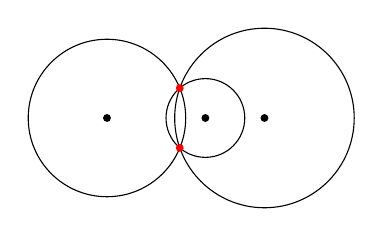
\begin{tikzpicture}
      \draw (0,0) circle (1cm); \fill[black] (0,0) circle (0.05cm);
      \draw (1.25,0) circle (0.5cm); \fill[black] (1.25,0) circle (0.05cm);
      \draw (2,0) circle (1.14cm); \fill[black] (2,0) circle (0.05cm);
      \fill[red] (0.925,0.3795) circle (0.05cm);
      \fill[red] (0.925,-0.3795) circle (0.05cm);
     \end{tikzpicture}
     \caption{Trilateration: wrong placement}
     \label{fig:research:trilaterationWrong}
    \end{center}
   \end{minipage}
   \hfill
   \begin{minipage}[b]{.3\textwidth}
    \begin{center}  
     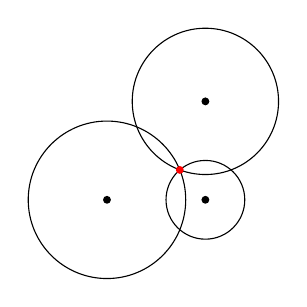
\begin{tikzpicture}
      \draw (0,0) circle (1cm); \fill[black] (0,0) circle (0.05cm);
      \draw (1.25,0) circle (0.5cm); \fill[black] (1.25,0) circle (0.05cm);
      \draw (1.25,1.25) circle (0.929cm); \fill[black] (1.25,1.25) circle (0.05cm);
      \fill[red] (0.925,0.3795) circle (0.05cm);
     \end{tikzpicture}
     \caption{Trilateration: right placement}
     \label{fig:research:trilaterationRight}
    \end{center}
   \end{minipage}
  \end{figure}\\
  As you can see on figure \ref{fig:research:trilaterationWrong}, the 3 points are not allowed to be on one line, a better approach is shown on figure \ref{fig:research:trilaterationRight}.
%%%%%%%%%%%%%%%%%%%%%%%%%%%%%%%%
%%%%% MATHEMATICAL SECTION %%%%%
%%%%%%%%%%%%%%%%%%%%%%%%%%%%%%%%
 \section[Mathematical fundamentals]{Mathematical fundamentals for location detection}
  \label{sec:research:math}
   This section describes how to calculate a trilateration.
% 1 DEVICE
  \subsection{One device}
   If there is only one device it would not be clear where exactly the person, which should be located, is. Only the distance to that specific device is known.\\
   \begin{figure}[h]
    \centering
    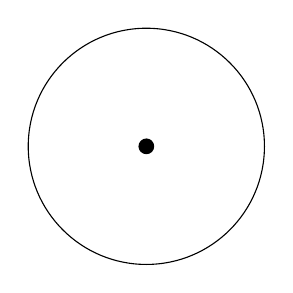
\begin{tikzpicture}
     \draw (0,0) circle (1.5cm);
     \fill[black] (0,0) circle (0.1cm);
    \end{tikzpicture}
    \caption[Only one device]{what it would look like if there would be only one device}
    \label{fg:only_one_device}
   \end{figure}\\
   As can be seen in figure \ref{fg:only_one_device} the person can be anywhere on the circle.

% 2 DEVICEs 
  \subsection{Two devices}
   If there were only two devices it would be much easier to clarify where the person is. The exact position is still not found, but instead of an infinite amount of possible positions it is reduced to 2 possible positions.

   \begin{figure}[h]
    \centering
    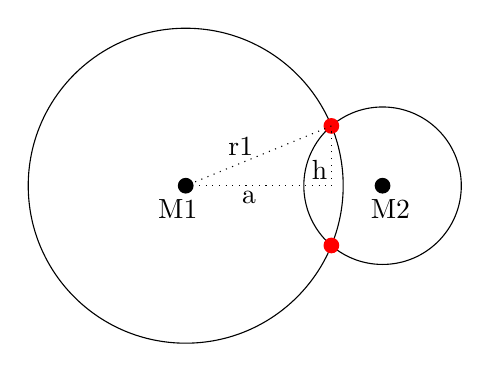
\begin{tikzpicture}
     \draw (0,0) circle (2cm); \fill[black] (0,0) circle (0.1cm);
     \draw (-0.1,-0.3) node {M1};
     \draw (2.5,0) circle (1cm); \fill[black] (2.5,0) circle (0.1cm);
     \draw (2.6,-0.3) node {M2};
     \fill[red] (1.85,0.759) circle (0.1cm);
     \fill[red] (1.85,-0.759) circle (0.1cm);
%	now the triangle:
     \draw[style=dotted] (0,0) -- (1.85,0);
     \draw (0.8,-0.15) node {a};
     \draw[style=dotted] (1.85,0) -- (1.85,0.759);
     \draw (1.7,0.2) node {h};
     \draw[style=dotted] (1.85,0.759) -- (0,0);
     \draw (0.7,0.5) node {r1};
    \end{tikzpicture}
    \caption[Only two devices]{what it would look like if there would be only two devices}
    \label{fg:only_two_devices}
   \end{figure}

   To obtain the positions of the red dots in figure \ref{fg:only_two_devices} one have to calculate using the following formulas: \\
   The given values are:\\
   Circle one: $x_1$, $y_1$, $r_1$\\
   Circle two: $x_2$, $y_2$, $r_2$\\
   Where $x_n$ and $y_n$ are the two coordinations of the circles and $r_n$ are the radii of the circles.
   At first the distance ($d$) between the two middle points needs to be calculated:

   \begin{eqnarray} \label{eq:distanceOfMiddlePoints}
    d_x = x_2 - x_1\\
    d_y = y_2 - y_1\nonumber\\
    d = \sqrt{ d_x^2 + d_y^2}\nonumber
   \end{eqnarray}

   If $d$ is zero then the two circles have the same middle point and either the two circles are identical or do not have any intersection points. After the distances between the two middle points is calculated the distance $a$ (see figure \ref{fg:only_two_devices}) needs to be calculated:

   \begin{equation}\label{eq:distanceA}
    a = \frac{r_1^2 - r_2^2 + d^2}{2*d}
   \end{equation}

   The last distance that need to be calculated is the height $h$ (see figure \ref{fg:only_two_devices}).

   \begin{eqnarray}\label{eq:height}
    h^2 = r_1^2 - a^2\\
    h = \sqrt{r_1^2 - a^2}\nonumber
   \end{eqnarray}

   The following table shows the characteristics of $h^2$.

   \begin{table}[h!]
    \centering
    \begin{tabular}{l|l}
     $h^2 < 0$ & no intersection point\\
     $h^2 = 0$ & exactly one intersection point\\
     $h^2 > 0$ & two intersection points with the distance $2*h$\\
    \end{tabular}
    \label{tb:research:math:heightCharacteristics}
    \caption{$h^2$ Characteristics}
   \end{table}

   After the height is calculated the coordination(s) of the intersection point(s) can be calculated:

   \begin{eqnarray}\label{eq:intersectionCoordination1}
    xi_1 = x_1 + \frac{a}{d}*d_x - \frac{h}{d}*d_y\\
    yi_1 = y_1 + \frac{a}{d}*d_y + \frac{h}{d}*d_x\nonumber
   \end{eqnarray}

   \begin{eqnarray}\label{eq:intersectionCoordination2}
    xi_2 = x_1 + \frac{a}{d}*d_x + \frac{h}{d}*d_y\\
    yi_2 = y_1 + \frac{a}{d}*d_y - \frac{h}{d}*d_x\nonumber
   \end{eqnarray}

   Equation \ref{eq:intersectionCoordination1} shows how the first intersection point is calculated and \ref{eq:intersectionCoordination2} how the second. \citep{MartinKowalski:CircleIntersection}

% 3 DEVICES
  \subsection{Three devices}
   Finally if there are 3 devices it is possible to detect the correct position of the person to locate.
   \begin{figure}[h]
    \centering
    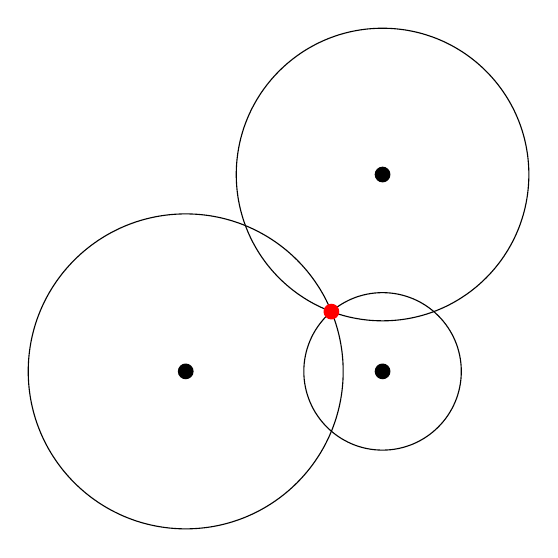
\begin{tikzpicture}
     \draw (0,0) circle (2cm); \fill[black] (0,0) circle (0.1cm);
     \draw (2.5,0) circle (1cm); \fill[black] (2.5,0) circle (0.1cm);
     \draw (2.5,2.5) circle (1.858cm); \fill[black] (2.5,2.5) circle (0.1cm);
     \fill[red] (1.85,0.759) circle (0.1cm);
    \end{tikzpicture}
    \caption[Three devices]{what it would look like if there would be three devices}
    \label{fg:three_devices}
   \end{figure}\\
   To calculate the location of the red dot in figure \ref{fg:three_devices}, the previously created equations, \ref{eq:intersectionCoordination1} and \ref{eq:intersectionCoordination2}, for getting the coordinates of the two intersection points will be needed. Both have a maximum of two results, which will result into $\left(xi_1,yi_1\right)$ and $\left(xi_2,yi_2\right)$. Now the only test that needs to be performed is checking which of those two points is on the third circle. The formula for calculating this is as follows:\\

   First calculate the distance from the circles middle $M\left(M_x,M_y\right)$ to the point $P\left(X,Y\right)$.
   \begin{equation} \label{eq:threeCirclesTest}
    d = \sqrt{\left(X-M_x\right)^2+\left(Y-M_y\right)^2}
   \end{equation}
   Then compare the distance $d$ with radius $r$ of the circle, if $d < r$ then the point is in the circle, if $d > r$ then the point is not in the circle and if $d = r$ then the point is on the circles border.
%%%%%%%%%%%%%%%%%%%%%%%%%%%%%%%%%%%%%%%%%%%
%%%%% Technologies and their Hardware %%%%%
%%%%%%%%%%%%%%%%%%%%%%%%%%%%%%%%%%%%%%%%%%%
 \section{Technologies and their Hardware}
  This section will cover a few technologies that can be used for location detection. The described technologies are limited to those who are easy working with a common personal computer.

  \subsection{WLAN}
   Wireless Local Area Network (WLAN) is commonly used for computers and other devices that need access to a Local Area Network (LAN). Mostly it is build up with access points, on which every wireless device must register. The communication is mostly driven over the 5 GHz and the 2.4 GHz public spectrum bands (see IEEE 802.11).

   The access points have several information about every device that is registered with them. One of the useful information are the MAC address and the sending strength. With the MAC address every registered device is explicitly identifiable, because every device should have a unique MAC address on the world. With the sending strength it is possible to find out how big the distance between the access point and the device is. The position accuracy of the devices is very high, around $10cm$.

   To get information about the strength of the signal, the access points must have the ability to display it. In most cases access points do not have this ability with their default firmware, therefore the access points needed to get flashed with a new operating system. After flashing the access points are getting the ability to run custom software. This Software can be used to provide the requested data upon the signal strength. Those operating systems are mostly build on top of a small Linux and extend the original features considerably.

   An example for such a firmware is dd-wrt (\url{http://www.dd-wrt.com/}). Dd-wrt provides access through a web interface as well as through a console using the ssh protocol. The console interface enables the use of self written programs, which then can use the router for their own needs. The console also allows the administrator to configure or to install new packages on the router.

   To make location detection possible with the WLAN technology the following parts are needed. Like already explained in \ref{sec:research:math}, three receiving devices are needed. At the WLAN technology those receiving devices are the access points. Suitable devices for clients are all devices that can connect to an access point, like mobile phones, PDAs and notebooks.

  \subsection{Bluetooth}
   Bluetooth was constructed as a low powered wireless connection. It is mainly used for applications that do not use a very high bandwidth. The Bandwidth varies in each standard, Bluetooth 1.0 has about 721 kbit/s and Bluetooth 2.0 has around 2.1 mbit/s.

   The main application area are transmissions between mobile phones and communication between the peripheral computer hardware and the computer itself.

   Like above in the WLAN section, we again need three devices that are capable of receiving Bluetooth signals and have the capability of getting attached to a computer. Additional to the receiving devices the project would be in need of a device that will act as a client, which sends a signal to the master device. The master devices are mostly called dongles, those are small device which are connected to the computers USB port. A master device can handle a maximum of 7 clients, so building up a detection network can become complex if the number of clients is larger than 7 \citep[p.18--27]{NathanJMuller:2002}. Possible client devices again are mobile phones, PDAs and notebooks.

   The costs of building a network on top of the Bluetooth technology would be a little cheaper than the WLAN approach, as long as the number of clients is less than or equal to 7. If there are more than 7 clients this solution will become  more expensive.

  \subsection{RFID}
   The Radio-Frequency Identification (RFID) technology is separated into two main areas of RFID chips (further more called tags). The first area is using passive tags the second one uses active ones. Passive tags do not have a power supply and only work through the short frequency impulse that hits them if a reader is trying to read the data that is stored on the chip. Because of that, the passive chips have only a very short range in which their data can be read, approximately 10 cm. The active chips on the other hand have their own power supply which gives them the opportunity to enforce the signal they are meant to send back to the reader. Those enforcement gives them the ability to broadcast their signal in a wider range than the passive ones, approximately 50 and more meters, depending on the attached power supply and the surroundings.

   Because of the fact that every tag answers every reader the tags do not need to register themself at the reader. The basic functionality is that the reader asks, by sending a specific signal on a specific frequency, all tags to answer him by sending their data back. Then all the tags that are in range will answer the sender by sending their data back to the sender.

   The hardware for this technology is not yet buyable in every store because its mainly used by the industry for logistic solutions, and there are no real suitable applications to the normal human being up to now. The expensive parts on this technology are still the readers, clients which are sending the signals are the way more cheaper than on WLAN or Bluetooth. The construction costs of passive tags are a few pennies, only the costs of active tags is higher and is about 20 \pounds.

  \subsection{ZigBee}
   The following information are taken from the official ZigBee Specification \citep{Various:ZigBee} as well as some online technology specifications provided on wikipedia \citep{wikipedia:ZigBee}.

   ZigBee is a technology that was developed by the industry to have an ``simple, just working'' low-cost wireless technology. These wireless connections should be used by any devices that need to connect to each other. Those devices are those used in the industry as well as home devices. The ZigBee technology is an advancement of the WLAN and the Bluetooth technologies. The signal ranges are pretty much the same as those from WLAN and it is using the 2,4 GHz spectrum band. 

   The ZigBee network is using three different types of devices in its network structure.
   \begin{itemize}
    \item The \textbf{ZigBee coordinator (ZC)} is used as the coordinator of a whole network. It has also the capability of bridging the traffic into other networks.
    \item The \textbf{ZigBee Router (ZR)} is capable of being used as end device but also can send data to other routers or the coordinator.
    \item The \textbf{ZigBee End Device (ZED)} is the device which is used in applications, it does not have the capability to relay data, it only can communicate with routers or the coordinator.
   \end{itemize}

   Those technology is mostly used by the industry for industrial use, therefore the devices are not purchasable on every store.

  \subsection{Conclusion}
   ZigBee might have been the best choice for this project, because the parts are cheap and yet well elaborated. But the problem is that it is not easy to get parts for such a small project like this one.

   \begin{table}[h!]
    \begin{minipage}{\textwidth} 
     \centering
     \footnotesize
     \begin{tabular}{|l|c|c|c|c|c|c|}
      \hline
       Technology& Range	& Accuracy	&Transfer rate		&\multicolumn{2}{|c|}{Prizes\footnote{all prizes are approximated }}&Overall\\
		&		&		&			& tag	& node	& rating\\
      \hline
      \hline
       Bluetooth& $8m$		& $\pm$5m	& 2.1 Mbit/s\footnote{In Version 2}, & $\>$ 100\textgreek{\euro}(70\pounds)& 11\textgreek{\euro}(8\pounds)	& *\\
       		&		&		& 480 Mbit/s\footnote{In Version 3} & & &\\
      \hline
       WLAN	& 10-100m	& $\pm$10cm	& 1-108 Mbit/s	& $\>$ 100\textgreek{\euro}(70\pounds)& 50\textgreek{\euro}(35\pounds)	& ***\\
      \hline
       RFID	& 10-80m	& $\pm$10cm	& $<$ 20 Kbit/s& 20\textgreek{\euro}(15\pounds)& 85\textgreek{\euro}(60\pounds)	& *****\\
      \hline
       ZigBee	& 10-100m	& n/a		& 20-250 Kbit/s	& $<$5\textgreek{\euro}(3.5\pounds)& $<$5\textgreek{\euro}(3.5\pounds)& ****\\
      \hline
     \end{tabular}
     \label{tab:technologies}
    \end{minipage}
    \caption[Technology statistics]{Technology statistics (1 * is low, 5 are high)}
   \end{table}

   Table \ref{tab:technologies} shows the key values of each technology and an overall rating done by the developer. The Rating is based on how the technology will fit into the given parameters, like having a good accuracy. The accuracies were measured by the developer. Because he did not have any ZigBee technology the accuracy of this technology could not be tested. But like written in the above statement the ZigBee technology was separated from the project as soon as it was evident that the needed parts are not easy purchasable.

   Both the Bluetooth and the WLAN technology were not chosen because they both have no ``independent sending-only'' tags. Which means that the user who wants to be located needs at least a mobile phone or a PDA with those capabilities for detection. Both devices are not very cheap and both are way to big to carry around.

   Those facts and the fact that the RFID technology is a relatively new and interesting technology made the decision, that it would be nice to develop the system on top of the RFID technology. Anyway the system should be designed to easily adapt other technologies by simply implementing the interface for the other hardware.

%%%%%%%%%%%%%%%%%%%%%%%%%%%%%%%%%%%%%%%%%%%
%%%%%        CHOSEN HARDWARE          %%%%%
%%%%%%%%%%%%%%%%%%%%%%%%%%%%%%%%%%%%%%%%%%%
  \subsection{Chosen Hardware}
   After some searches for suitable hardware, the OpenBeacon project (\url{http://www.openbeacon.org/}) was found. This project provides both needed parts for the location detection.

   \subsubsection*{Tag}
    The tags are small round electronic units with the following measurements:
    \begin{table}[h]
     \centering
     \begin{tabular}[h]{|l|l|}
      \hline
       \textbf{Diameter:}	& $3.5 cm$\\
      \hline
       \textbf{Depth:}		& $0.7 cm$\\
      \hline
     \end{tabular}
     \caption{Dimensions of CCC Sputnik RFID tag}
     \label{tab:beacon_dimensions}
    \end{table}

    \begin{figure}[h]
     \begin{minipage}[b]{.5\textwidth}
      \centering
      \includegraphics[scale=0.8]{images/tag_front.png}
      \caption{Front of CCC Sputnik RFID tag}
      \label{fg:tag_front}
     \end{minipage}
     \begin{minipage}[b]{.5\textwidth}
      \centering
      \includegraphics[scale=0.8]{images/tag_back.png}
      \caption{Back of CCC Sputnik RFID tag}
      \label{fg:tag_back}
     \end{minipage}
    \end{figure}

    Figure \ref{fg:tag_front} shows the front of the selected hardware tag. This specific tag has an additional function which allows to send a press of a button to the receivers and on figure \ref{fg:tag_back} the battery case with the imprinted tag id are well visible.

    The tag needs a CR 2032 Battery with $3V$. The battery will not be replaced for approximately one year. The tag has also a small little light emitting diode (LED) which blinks around every second to show that the tag is working and sends data.

   \subsubsection*{Reader}
    The OpenBeacon project also supplies an adequate reader that uses the USB port to provide the data. The dimensions\footnote{Height and depth might change when antenna is applied and turned in some way} of the OpenBeacon USB node are shown in table \ref{tab:tag_dimensions}.
    \begin{table}[h]
     \centering
     \footnotesize
     \begin{tabular}[h]{|l|l||l|l|}
      \hline
       \multicolumn{2}{|c||}{Node}				& \multicolumn{2}{|c|}{Antenna}\\
      \hline
      \hline
       \textbf{Width:}	& $7.5 cm$ 				&\textbf{Length:}	& $9.7 cm$\\
			& $\sim 8 cm$ with an applied antenna	&			& \\
      \hline
       \textbf{Height:}	& $2.5 cm$				&\textbf{Diameter:}	& $1 cm$ \\
      \hline
       \textbf{Depth:}	& $1.2 cm$				&\textbf{Socket length:}& $1.7 cm$\\
      \hline
			&					&\textbf{Socket diameter:} & $1 cm$\\
      \hline
     \end{tabular}
     \caption{Dimensions of OpenBeacon USB hardware}
     \label{tab:tag_dimensions}
    \end{table}

    \begin{figure}[h]
     \begin{minipage}[b]{.5\textwidth}
      \centering
      \includegraphics[scale=0.6]{images/beacon_front.png}
      \caption{Front of OpenBeacon USB node}
      \label{fg:beacon_front}
     \end{minipage}
     \begin{minipage}[b]{.5\textwidth}
      \centering
      \includegraphics[scale=0.6]{images/beacon_back.png}
      \caption{Back of OpenBeacon USB node}
      \label{fg:beacon_back}
     \end{minipage}
    \end{figure}

    Figure \ref{fg:beacon_front} shows the upper side of the OpenBeacon USB node on the left end is the connector to the $2,4 GHz$ antenna and on the right side is the USB port. Figure \ref{fg:beacon_back} shows the back of the OpenBeacon USB node. Both figures show the unattached $2,4 GHz$ antenna on the bottom. The antenna itself has a free turnable joint which allows the user to turn the antenna in different directions when it is applied to the node.

   To perform the location detection there are two of the tags and three reader. This project needs two tags to have the possibility to check what happens if more than one tag is in range.

  \subsubsection{Changes to operating system}
   To operate with the hardware the operating systems needed a few changes and a new set of tools to communicate with the reader.

   \subsubsection{Kernel changes}
   \label{sec:research:KernelChanges}
    First thing that had to be changed was the kernel. This needed to be done to let any kind of software address the hardware and talk to it, therefore a device was added. The device that was needed for the USB reader is a serial USB device in this case an abstract control model (ACM) device. If the kernel module cdc-adm is not already available, then the kernel needs to be rebuild with the enabled option.

    To enable USB ACM support. the following needs to be marked as module or built in:

    \begin{lstlisting}[frame=single,breaklines,basicstyle=\footnotesize,label=lst:kernelEnableACM,captionpos=b,caption={Where to enable ACM support}]
Device Drivers
   -> USB Support
      -> Support for Host-side USB
         -> USB Modem (CDC ACM) Support
    \end{lstlisting}

    If it was build as a module then it would help to simply start the module by entering \verb modprobe  \verb cdc-acm  and if it was built in the computer needed to be restarted to load the new kernel. After that is done a device will show up as soon as the OpenBeacon USB node is plugged into a free USB port. The upcoming devices name will be \verb /dev/ttyACM? . The ? stands for the number of the device.

    To \textbf{flash} the reader with a new firmware, the operating system is in need of an USB serial device. If the usbserial module does not exists the following must be set to module or built in.

    \begin{lstlisting}[frame=single,breaklines,basicstyle=\footnotesize,label=lst:kernelEnableUSBSerial,captionpos=b,caption={Where to enable USB serial}]
Device Drivers
   -> USB Support
      -> USB Serial Converter support
         -> USB Serial Converter support
    \end{lstlisting}

    Again if it was as module just load it with \verb modprobe  \verb usbserial  or restart the computer to enable the new kernel. When the computer booted again plug in the reader and as soon it is plugged in there should be a device called \verb /dev/ttyUSB? . Again the ? stands for the number of the device. If the device does not show up then the systems device manager is not configured to handle the USB serial module. To configure this right the following must be done as root:\\

    \begin{lstlisting}[frame=single,breaklines,basicstyle=\footnotesize,label=lst:usbserialUdevRule,captionpos=b,caption={How to enable usbserial in udev}]
$ echo "BUS==\"usb\", KERNEL==\"ttyUSB*\", GROUP=\"uucp\", MODE=\"0666\"" >> /etc/udev/rules.d/10-custom.rules
$ echo "BUS==\"usb\", KERNEL==\"ttyACM*\", GROUP=\"uucp\", MODE=\"0660"" >> /etc/udev/rules.d/10-custom.rules
$ udevstart
    \end{lstlisting}
    After this the reader needs to plugged out and re plugged in and the modules needs to be reloaded. if the device still not show up the following needs to be done, as root again:
    \begin{lstlisting}[frame=single,breaklines,basicstyle=\footnotesize,label=lst:usbserialModprobe,captionpos=b,caption={How to modprobe usbserial}]
$ lsusb
 Bus 001 Device 001: ID 0000:0000
 Bus 002 Device 004: ID 03eb:6124 Atmel Corp.
 Bus 002 Device 002: ID 04f3:0210 Elan Microelectronics Corp.
 Bus 002 Device 001: ID 0000:0000
$ modprobe usbserial vendor=0x03eb product=0x6124
    \end{lstlisting}
    The output from \verb lsusb  should show an Atmel Corp. device. The first number before the colon is the vendor id the one after it is the product id. If they differ, the modprobe call needs to be adjusted appropriate. After all that work the reader is ready to get flashed.

   \subsubsection{Tools}
    In order to flash the OpenBeacon node with a new firmware version the Linux operating system needed to be extended by the following tools:
    \begin{itemize}
     \item A compiler to build firmware binaries that could run on the OpenBeacon node. The compiler used is the gcc-arm, this special version of the gcc produces binaries for the arm processor.
     \item A tool to write the binary firmware file on the OpenBeacon node, those tools are normally called flash tools. The flash tool that was used for this project is a modified version from the OpenPCD (\url{http://www.openpcd.org/}) project that comes from the same supplier as the OpenBeacon project. Those flash tools are available from here: \url{http://www.openpcd.org/dl/sam7utils-0.1.0-bm.tar.bz2}.
    \end{itemize}
    There are only three steps needed to flash a new firmware on the OpenBeacon node.
    \begin{enumerate}
     \item \textbf{Create and compile new Firmware}\\
      Change or create new firmware and compile it with the gcc-arm compiler.
     \item \textbf{Delete the current Firmware}
      To delete the firmware the node needs to be unplugged, then a jumper needs to be placed on the two pins. The second step is to plug the node back into the USB port of a running computer. After 10 seconds the current firmware will be deleted and the node needs to pulled out. After the jumper is removed the node can be plugged back into the USB port again. Now a \verb lsusb should show something like it is shown in listing \ref{lst:usbserialModprobe}.
     \item \textbf{Flashing the OpenBeacon node}
      If there is no \verb /dev/ttyUSB0 then the \verb modprobe command from listing \ref{lst:usbserialModprobe} should be used to create it. After the device shown up the at91flash script (delivered with the original firmware) should be used to flash the device. As soon as the flashing is done the last task is to unplug and re-plug the device to let the computer take notice that the device has changed.
    \end{enumerate}
%%%%%%%%%%%%%%%%%%%%%%%%%%%%%%%%%%%%
%%%  Analysis of the technology  %%%
%%%%%%%%%%%%%%%%%%%%%%%%%%%%%%%%%%%%
 \subsection{Analysis of the technology}
  \subsubsection*{How does the hardware work}
   When the hardware is plugged in and the operating system is configured right, it can be tested with the \verb cu program from Taylors UUCP package. The connection can be made with the following command:
   \begin{lstlisting}[frame=single,breaklines,basicstyle=\footnotesize,label=lst:cuCommand,captionpos=b,caption={cu command to access OpenBeacon node}]
$ cu -lttyACM0 -s 115200
 RX: 0,2213,8
 RX: 0,2213,8
 RX: 0,2213,8
 RX: 0,2213,8
 RX: 0,2213,9
 RX: 0,2213,9
 RX: 0,2213,9
 RX: 0,2213,9
   \end{lstlisting}
   As shown in listing \ref{lst:cuCommand} the information from the OpenBeacon node is starting right after it is connected. Each line provides the following information (in that order):
   \begin{enumerate}
    \item \textbf{RX} to show that this is a received information from a tag
    \item The \textbf{first number} is the lowest strength on which the signal is received, it can be one of the following: 0, 85, 170, 255.
    \item The \textbf{second number} is the id of the tag to which the received information belong.
    \item The \textbf{last number} is the amount of received packages, in this example the maximum are 10 packages.
   \end{enumerate}
   This was the first thing that was different than expected. Expected was that the OpenBeacon and the tags would deliver the signal strength but this was a wrong assumption. But it should be no problem to implement a location system based on the packet loss distance retrieving described in section \ref{sec:research:locdetection}. Figure \ref{fg:research:numberRayOrig} shows a number ray of the strength values and how they relate to the distance from the tag to the node.
   \begin{figure}[h!]
    \centering
    \begin{tikzpicture}
     \draw (-1,1) node {Near};
     \draw (9,1) node {Far};
     \draw (-1,0) -- (10,0);

     \draw (0,-1) -- (0,1);
     \draw (1,1) node {0};
     \draw (1,-1) node {10\dots0};

     \draw (2,-0.5) -- (2,0.5);
     \draw (3,1) node {85};
     \draw (3,-1) node {10\dots0};

     \draw (4,-0.5) -- (4,0.5);
     \draw (5,1) node {170};
     \draw (5,-1) node {10\dots0};

     \draw (6,-0.5) -- (6,0.5);
     \draw (7,1) node {255};
     \draw (7,-1) node {10\dots0};

     \draw (8,-1) -- (8,1);
    \end{tikzpicture}
    \caption{Number ray of the original strength values}
    \label{fg:research:numberRayOrig}
   \end{figure}\\

   To make an easier location detection the absolute strength will be calculated with the following formula: $\textrm{strength} = \frac{\textrm{power level}}{85} * 10 + \left(\textrm{maximum packages} - \textrm{packet loss}\right)$. Figure \ref{fg:research:numberRayWithFormula} shows a the number ray with the effect the formula gives to the original strength number ray.\\

   \begin{figure}[h!]
    \centering
    \begin{tikzpicture}
     \draw (-1,1) node {Near};
     \draw (9,1) node {Far};
     \draw (-1,-2) node {Strength};
     \draw (5,-2) node {0\dots40};
     \draw (-1,0) -- (10,0);

     \draw (0,-1) -- (0,1);
     \draw (1,1) node {0};
     \draw (1,-1) node {0\dots10};

     \draw (2,-0.5) -- (2,0.5);
     \draw (3,1) node {85};
     \draw (3,-1) node {0\dots10};

     \draw (4,-0.5) -- (4,0.5);
     \draw (5,1) node {170};
     \draw (5,-1) node {0\dots10};

     \draw (6,-0.5) -- (6,0.5);
     \draw (7,1) node {255};
     \draw (7,-1) node {0\dots10};

     \draw (8,-1) -- (8,1);
    \end{tikzpicture}
    \caption{Number ray of the strength values after using the formula}
    \label{fg:research:numberRayWithFormula}
   \end{figure}

   The OpenBeacon node firmware also provide some configuration functionalities. The help screen, will show up as soon as the user types \verb=?= or \verb=h= followed by enter.
   \begin{lstlisting}[frame=single,breaklines,basicstyle=\footnotesize,label=lst:openBeaconHelpScreen,captionpos=b,caption={Console output of the help screen}]
RX: 0,2213,9
RX: 0,2213,9
Command received:?
 *****************************************************
 * OpenBeacon USB terminal                           *
 * (C) 2007 Milosch Meriac <meriac@openbeacon.de>    *
 *****************************************************
 *
 * S          - store transmitter settings
 * C          - print configuration
 * I [id]     - set reader id
 * FIFO [sec] - set FIFO cache lifetime in seconds
 * 0          - receive only mode
 * 1..4       - automatic transmit at selected power levels
 * ?,H        - display this help screen
 *
 *****************************************************
   \end{lstlisting}
   The help screen from listing \ref{lst:openBeaconHelpScreen} shows that it is possible to change a few settings that will be needed by the project.
   \begin{lstlisting}[frame=single,breaklines,basicstyle=\footnotesize,label=lst:openBeaconSettingsScreen,captionpos=b,caption={Console output of the settings screen}]
RX: 0,2213,9
RX: 0,2213,9
Command received:C
 *****************************************************
 * Current configuration:                            *
 *****************************************************
 *
 * Uptime is 0h:4m:37s
 * The reader id is 1
 * The mode is 1
 * The channel is 81
 * The FIFO cache lifetime is 10s
 *
 *****************************************************
   \end{lstlisting}
   The listing \ref{lst:openBeaconSettingsScreen} shows the settings screen. It displays the uptime, the id of the reader (it can be between 0 and 255), the mode (0 if it is in receiving mode, 1 to 4 for the power levels of sending), the channel and the lifetime of the package cache.
   
  \subsubsection*{Missing firmware capabilities}
   As shown in the listings \ref{lst:openBeaconSettingsScreen} and \ref{lst:openBeaconHelpScreen} it is not possible to retrieve information on a single output line. Therefore the project needs to enhance the firmware with the following abilities:
   \begin{itemize}
    \item Retrieving information on a single line for easier parsing of information like the id.
    \item It also misses some range queries, it should ask if the number of the id is higher than 255. At the moment it allows nearly every number, but this can be dangerous because with to high numbers the memory after the number can be lost (buffer overflow)
   \end{itemize}
%%%%%%%%%%%%%%%%%%%%%%%%%%%%%%%%%%%%%%%%%%%%%%%%%%%%%%%%
%%%    Writing a prototype to access the Hardware    %%%
%%%%%%%%%%%%%%%%%%%%%%%%%%%%%%%%%%%%%%%%%%%%%%%%%%%%%%%%
 \subsection{Writing a prototype to access the Hardware}
  This prototype should be used to find out how much work it will be to make the hardware work and with which commands it can be accessed. Basicly it should do all the basic things that can \verb cu do, connect, read, write and disconnect. It will not have much error handling or checks if the user used the program in the right way.
  \subsubsection*{Basic design}
   Basicly the prototype consists of two modules.
   \begin{enumerate}
    \item The first module would be the main module it opens the port to the hardware and will listen to it. Everything that is read from the OpenBeacon node will be printed to the screen. It will also listen to a message queue for incoming commands from the user. As soon as some commands are coming in the main module should send them to the node. Then the results should be printed, like all information that is coming from the hardware.
    \item The second module is the controlling unit, whilst the first module just prints everything it gets from the OpenBeacon node, this second module has the capability to give the first module orders. Those orders are send through a message queue and are just the same commands like displayed in the help screen you can see in listing \ref{lst:openBeaconHelpScreen} with an additional command to let the module quit. The commanding module will only send a command and afterwards it quits, if the user wants to send more than one command, the module has to be called more than once.
   \end{enumerate}
   Both Modules are running on the console only, there will be no graphical user interface.

  \subsubsection*{Outcome}
   The full source code and build file can be found on the delivered CD as well as in appendix \ref{app:prototypeCode}. One of the base concept of all UNIX like systems is that ``\textit{Everything is a file}``. In close that means that a program can access a system device like it can access a file. That is the reason why it was so easy to create the prototype, there are only a few basic functions needed to work with the OpenBeacon device.
   \begin{itemize}
    \item The \textbf{open} instruction opens a file or device and returns a file descriptor which then can easily used by the other three commands. (An example can be found on listing \ref{lst:prototypeMain} in the appendix \ref{app:prototypeCode} at line 26)
    \item The \textbf{read} instruction reads bytes from the file descriptor, the command can read only a specified amount of data. (Listing \ref{lst:prototypeMain} in the appendix \ref{app:prototypeCode} at line 60)
    \item With the \textbf{write} command the program can write bytes to the file descriptor. (Listing \ref{lst:prototypeMain} in the appendix \ref{app:prototypeCode} at line 81)
    \item The \textbf{close} instruction is used to close the file descriptor after it is no longer of use. (Listing \ref{lst:prototypeMain} in the appendix \ref{app:prototypeCode} at line 91)
   \end{itemize}
   Detailed information to each of those commands can be found in the manual pages of the Linux operating system.
%%%%%%%%%%%%%%%%%%%%%%%%%%%%%%%%%%%%%%%%%%%
%%%%%        Operating systems        %%%%%
%%%%%%%%%%%%%%%%%%%%%%%%%%%%%%%%%%%%%%%%%%%
 \section{Operating systems}
  \label{sec:research:operationSystems}
  This section will cover the basic two operating systems that could have been used to realize this project. The developer needs to know which operating system the development will be done to verify that the hardware which will be used is able to work with it.
  This section will give a short overview over Microsoft Windows and Linux.

  \subsection{Microsoft Windows}
   Microsoft Windows is one of the most used desktop operating systems in the world. It has a graphical user interface and a not very powerful command shell. Most of the software that is provided for MS Windows must be purchased, but many open source projects have windows ports so they can run there as well. A big advantage of Microsoft Windows is that most of the software that is available for Windows is easy install-able and works right out of the box, but as soon as something is not happening like it should be it is not so easy to figure out what is cousing the problem. A big disadvantage of this operating system is that on every new release the end user has to buy the new version. The EULA from Microsoft Windows limits its users in a lot of ways like it forbids the multiple installation on various self owned machines, every machine needs is own licence.

  \subsection{Linux}
   Linux is an open source operating system initially created by Linus Torvalds. Nowadays there are several thousand people who develop for Linux and tools that run on Linux. Linux itself is just the kernel which brings up the system. The kernel also provides an easy to use interface to the hardware of the system. On top of it, programs will handle the user input. This input can be made on the console or on a graphical user interface. To get a graphical user interface the system needs an X Window system and a desktop environment that is running on top of it. The console or shell on Linux is a very powerful tool, because nearly everything that can be done in the graphical interface can also be done in the console. A big advantage for developers is that Linux provides a lot of library's to speak to hardware. A big disadvantage is that many software companies do not support Linux due to a binary incompatibility of those systems. Most of the tools that are used in Linux are free to install and use.

  \subsection{Conclusion}
   This project will make use of the Linux operating system. This decision was made with having in mind that searching for errors regarding device drivers are much easier to find in Linux than they will be found in Microsoft Windows. Another reason for this decision is that the developer is working best in the operating system that the developer is using at home or for personal use. Linux is even a good choice if the costs of the project should be kept low because most of the software that will be used is open source and therefore it is free of charge. This will lower the costs of the project only to the parts that need to be bought to achieve the location detection. The operating system and the development tools are free of charge and the computer on which the software will be developed is already existent.

%%%%%%%%%%%%%%%%%%%%%%%%%%%%%%%%%%%%%%%%%%%%%%%
%%%%%            Licences                 %%%%%
%%%%%%%%%%%%%%%%%%%%%%%%%%%%%%%%%%%%%%%%%%%%%%%
 \section{Licences}
  There are a lot of licences, nearly every company has its own licences and copyright on their code, that allows or disallows several things. Most of the free open source software's (FOSS) have licenses as well. This section will cover a few of them. The most famous one is the GNU General Public Licence (GPL), it is widely spread and a lot of well known projects like the Linux kernel or the K Desktop Environment (KDE) are using it. It allows other people to see, even change the code, but only if they are too publishing their source under the GPL. The developer is allowed to charge people for his effort in writing the source but he has to publish the source as well.\\

  Another Licence that will take effect in this project is the Q Public License Version 1.0, the official Qt (for more information regarding Qt reed section \ref{sec:research:programmingLanguages}) licence. This licence allows every developer to use this library without charge as long as he reveals the whole project code as well. If the developer wants to take money for his effort then he/she has to pay for the Qt library as well.

  For further information upon the Open source licences visit the Open Source Initiative licences web page \url{http://www.opensource.org/licenses/alphabetical}.
%% TODO: LGPL, BSD
  \subsection{Conclusion}
   This project will use the GPL to protect the sources and the developer who wrote them. By putting the source under the GPL it allows other developers to use it and change it for their own needs. After the project is done it will be released to the public so they can use it if they want to. Putting the RFID domestic location detection project under the GPL will also help with the spreading of the technology and the idea of using it in another way than it was planned to be.
%%%%%%%%%%%%%%%%%%%%%%%%%%%%%%%%%%%%%%%%%%%%%%%
%%%%% Programming languages and libraries %%%%%
%%%%%%%%%%%%%%%%%%%%%%%%%%%%%%%%%%%%%%%%%%%%%%%
 \section{Programming languages and libraries}
 \label{sec:research:programmingLanguages}
  This section will handle the choice of the programming languages and will describe why others were not taken. It will also give a short overview of the Qt library.\\

  C and C++ were chosen, because they are fast and have the ability to work close to the underlying hardware.
  Qt on the other hand is a great and well thought out set of classes that will help to concentrate the programming on the main tasks. Qt provides a set of standard functionalities like strings, lists, maps and even some communication classes like TCP/IP or UDP network or D-Bus (more on this in section \ref{sec:research:ipc}) inter process communication (IPC). The implementations of strings, lists and maps are significantly better than those from the Standard Template Library (STL). In addition to a good threading support, it also includes a wide set of graphical user interface classes.

  Qt's event system is also a well thought out system, instead of handling messages like it is done in other library's, it has a signal slot system. This signal slot system is a very powerful mechanism. If for instance a button is pressed in a GUI, a signal is invoked, now all previously connected slots (methods of the same or from other classes) will be executed. This system is not only working for the GUI, it will also work within all classes Qt provides as well as all project classes that will be need such a functionality.

  Another big advantage of Qt is its cross platform compatibility, which lets it run on at least Windows, Mac OS X and Linux. So applications written in Qt, are easy portable. Additional information can be found on the Qt web site \url{http://trolltech.com/}.\\

  %TODO: statt mfc .NET
  Other Library's like the Microsoft Foundation Classes (MFC) or C\# do not have much of the above mentioned features, and a big disadvantage is that they do not have the ability to run on other systems than windows.\\

  Java as an alternative programming language has more disadvantages than advantages for this project. The advantages are that the code is easily ported to every system where Java will run on. The disadvantages are that it is necessary to have Java itself installed on the system as well as it is using a lot of memory when it is running. The virtual machine requires a lot of memory, or just allocates it to have it ready just in case the application would need it. Also the garbage collector is a nice thing to have but if the programmer can think of its own and knows how to handle memory well, he will not need it. As table \ref{tab:speedCompareLanguages} shows, Java consumes a lot more time than a plain C or C++ program. Those measurements were done with the Linux \verb=time= command and the sources can be found in appendix \ref{app:severalSourceCodes:timeTestSources}.\\
  \begin{table}[h]
   \begin{minipage}{\textwidth}
    \centering
    \begin{tabular}[h]{|l||l|l|l|}
     \hline
      \textbf{Time}	& \textbf{C}	& \textbf{C++}	& \textbf{Java}\\
     \hline
     \hline
      real time\footnote{Time that elapsed from invocation to termination}& 0m0.002s & 0m0.003s & 0m0.165s\\
     \hline
      user CPU time	& 0m0.001s	& 0m0.001s	& 0m0.100s\\
     \hline
      system CPU time	& 0m0.001s	& 0m0.003s	& 0m0.022s\\
     \hline
    \end{tabular}
   \end{minipage}
   \caption{Speed comparison of programming languages}
   \label{tab:speedCompareLanguages}
  \end{table}

  As web programming languages there will be used HTML and PHP. Both are capable of running on different operating systems or web servers. This enables flexibility to the end user who chooses for himself on which system he will put the web configuration interfaces. Another web programming language is ASP (Active Server Page). It is designed to run on Microsoft Servers. Even if it is possible to run ASPs on other systems it will never run as good as on Microsoft systems, because the support of other systems is not given through Microsoft, but through third party companies.

 \subsection{Closer description of chosen language and libraries}
  The main language that will be used in this project is C++, due to the easy handling with devices under Linux and due to the good speed advantage like shown in table \ref{tab:speedCompareLanguages}. To support C++ the Qt library will be used. Qt offers a lot of subclasses that make it easier to code in C++. In addition to the helping Qt classes, Qt also provides an easy signal slot mechanism to communicate between objects. Both topics will be described below.

  \subsubsection*{Useful Qt subclasses}
  \label{sec:research:usefullQtSubclasses}
   Qt is separated into several theme related parts.
   \begin{itemize}
    \item \textbf{Threading}\\
     Qt provides a threading system that is easy to use and has the same capabilities like a non threaded Qt application like the very usable signal and slot inter object communication (see section \ref{sec:research:signalSlot}). This allows a quick response from one thread to another.
    \item \textbf{QtCore}\\
     The QtCore class collection has all the standard base classes like the Qt String class QString or several types of lists, QList and maps, QMap. Those core classes are used in every other part of Qt and are building the fundament of the Qt library.
    \item \textbf{QtDBus}\\
     The QtDBus collection holds all classes and methods that are needed for the D-Bus IPC.
    \item \textbf{QtGui}\\
     The QtGui subsystem includes all classes that are used to create GUIs. it has the capability to create GUIs in the source code by just putting the several components together or just include static created (with the included Qt designer) user interfaces.
    \item \textbf{QtNetwork}\\
     This subsystem is the network system of Qt and includes a lot of functions that make it easier to work with network communications. It provides the standard UDP and TCP communication as well as encrypted communication through SSL or protocol specific communication like ftp or http.
    \item \textbf{QtOpenGL}
     This subsystem of Qt provides a set of functionality for OpenGL graphic handling.
    \item \textbf{QtScript}
     QtScript provides a powerful scripting language to those Qt applications that are in need of one.
    \item \textbf{QtSql}
     With QtSql the Qt library provides simple access to several databases. The type of database may be chosen at runtime. This option allows the user to have much more flexibility with using the application and does not force to use a specific product
    \item \textbf{QtSvg}
     The QtSvg facility provides Qt with the ability to create and display Scalable Vector Graphics (SVG).
    \item \textbf{QtTest}
     the QtTest subsystem provides classes which allow the developer to create unit tests. Those tests can be used to verify that parts of the new created classes are going well. If in a later stage of development a change will be made to an old class and the old class provides some unit tests, the developer has the ability to check if the new changes broke anything.
    \item \textbf{QtXml}
     The QtXml module provides handling of the Extensible Markup Language (XML), stream based reader and writer as well as an C++ implementation of the ``Simple API for XML'' (SAX) and the ``Document Object Model'' (DOM).
   \end{itemize}

  \subsubsection*{Qt's signal and slot inter object communication}
  \label{sec:research:signalSlot}
     Qt provides a very powerful system which enables a communication between several objects, called the signals and slots system. This system allows objects to send signals if something important or something which is interesting for other objects occurs. Those signals can be optionally connected to slots, but they do not have to be. If they are not connected they will be ignored by the application. But if they are connected other objects can immediately react to the event that happened in the other object. A signal can also be attached to multiple slots and vice versa.

     This key-system makes the big difference from most of the other development frameworks around.

%%%%%%%%%%%%%%%%%%%%%%%%%%%%%%%%%%%%%%%%%%%%%%%
%%%%%          CODE REPOSITORIES          %%%%%
%%%%%%%%%%%%%%%%%%%%%%%%%%%%%%%%%%%%%%%%%%%%%%%
 \section[Code Version Control Systems]{Comparison between various code version control systems}
 \label{sec:research:codeVersionControl}
  A code repository is a system that watches over the different versions of a software project. Those different versions are mostly called revisions. Every upload of changed code will be reflected in an increment of the revision number. Those systems help software developers in keeping track of their project sources. If for example a developer has programmed something wrong and the whole project is not working anymore then the developer can undo everything to the last submitted state that was working.\\

  The Concurrent Versions System (CVS) and Subversion (SVN) are both working with this type of mechanism. The big difference between those two is their handling of commits, whilst the CVS is uploading all the files that have changed, SVN is just uploading a difference file to the server. On the first look this is no big deal, but if the project has large data files greater than 100MB, the CVS will upload 100MB every time there was a little change even if the change was just two changed byte. SVN on the other hand would only upload a difference file which describes the difference. If now someone updates its version of the project only the difference would be retrieved, if this person uses CVS it has to download the whole file.\\

  There are even other advantages like the handling itself, for example the user of SVN has to authenticate himself only once at the server, after that login information will be stored at the local code repository. This helps keeping the commands, regarding this repository, simple.

  \subsection{Conclusion}
   This project will use the SVN code repository system because it fits well with the Software Project Management System that was chosen (see section \ref{sec:research:softwareProjectManagement} for more details). It is known to minimise the traffic it is generating and therefore will be perfect to send data to a server which is not located at the university and therefore has a slower data connection.
%%%%%%%%%%%%%%%%%%%%%%%%%%%%%%%%%%%%%%%%%%%%%%%
%%%%%          BUILD ENVIRONMENTS         %%%%%
%%%%%%%%%%%%%%%%%%%%%%%%%%%%%%%%%%%%%%%%%%%%%%%
 \section[Build environments]{Build environments}
  Build environments are used to automatically build a whole project. If they are more powerful, they can even find needed libraries and link them to the project. There are a lot of build environments, but on this section we are only looking on three of them, CMake, SCons and a plain makefile.\\

  \subsection{Plain makefile}
   The plain makefile is just a small script that is used to build the application out of the source. The other two build environments have more intelligence. Those have the ability to find needed library's and link them to the application. They also provide mechanisms to configure the build type of the application, if for example an application can be build with console, graphical or both interfaces this could be specified before building.\\

  \subsection{SCons}
   SCons on the other hand consists of a single script, which uses python (a cross platform scripting language) for the configuration and build tasks. It has a few special functions which detect libraries. Anyway a SCons construction file is a large file and for small projects this file is sometimes larger (in size) than the whole project. The building of such a construct file is much more complex and needs knowledge in python as well.\\

  \subsection{CMake}
   CMake in the end, built on top of easy readable configuration files and CMake modules. These modules are used to find the librarys that are needed for the project. The configuration file is an easy to create and read file, which uses the modules to find and link the librarys. None the less it has the ability to compile the source on several platforms, as long as the source is capable of doing it. CMake creates a makefile which then can be used to build the application. Additional to the easy producible and understandable configuration file CMake is also faster than the other two build environments.

   The new version of KDE (K Desktop Environment) is using CMake as its building environment and is heavily based on Qt (see section \ref{sec:research:programmingLanguages}), therefore the Qt integration in CMake is well structured and easy to handle \citep{AlexanderNeundorf:KDEtoCMake}.

  \subsection{Conclusion}
   All three building environments have their pros and cons, the plain makefile is easy to create but it is not very usable if it comes to automatic path finding for includes and libraries. It is also not able to be used on more than one platform and therefore the application needs a makefile file for each platform. SCons has the abilities to find the paths and libraries even on different platforms but it is complex and needs additional knowledge of a scripting language. Those arguments are making CMake the best choice, because it is usable on different platforms, it finds paths and libraries by its own and the syntax, even if it is a new one to learn, is clear structured, easy to learn and needs less space than the SCons script.

   Because of those arguments the project will make use of the CMake building environment.
%%%%%%%%%%%%%%%%%%%%%%%%%%%%%%%%%%%%%%%%%%%%%%%
%%%%%    SOFTWARE PROJECT MANAGEMENT      %%%%%
%%%%%%%%%%%%%%%%%%%%%%%%%%%%%%%%%%%%%%%%%%%%%%%
 \section{Software Project Management}
 \label{sec:research:softwareProjectManagement}
  Software Project Management systems are used to manage a whole project and everything that is useful to a project. Those systems provide a wide set of functions to have an overview and a view of the current state of the project. This project will make use of one of them to have an easy system to manage the project and all of its aspects. A bug and ticket system will help to not forget things that still need to be done. The system will also provide other interested people (like the supervisor) with an overview of the system. This section will give an overview over two web based systems, trac and dotproject.

  \subsection{trac}
   Trac (\url{http://trac.edgewall.org}) is a web-based software configuration management (SCM) combined with a web interface to the project related SVN (see section  \ref{sec:research:codeVersionControl}) repository.\\
   The functions trac provides are:
   \begin{itemize}
    \item \textbf{A project related Wiki}\\
     This wiki can be used to give more information regarding the project.
    \item \textbf{A time line}\\
     The time line system gives information about actions that have happened in the last few days. Those actions are updates to the source, creation of new tickets (see below), closing of tickets, edits on the wiki, solved milestones (see below) and much more
    \item \textbf{A road map}\\
     This road map shows all open milestones and information to those. Each milestone has a percentage bar below its name which shows how far the milestone is done. The information to each milestone can be set by the developer, so it can be used to tell the current status as well as giving information about special bug fixes or workarounds.
    \item \textbf{A source browser}\\
     The source browser is a web-interface to the project related SVN repository. It can be used to browse the source and it has the possibility to show changes which were made between several revisions.
    \item \textbf{A complex ticket system}\\
     This ticket system is a big advantage of trac. Those tickets can be used to submit bugs or wishes. The tickets are assigned to several components and versions of the project and can have configurable statuses. The developer can even open tickets to show which tasks he has to solve before a milestone is done. Once a ticket is created all people have the ability to comment on the ticket or attach more information to it, but only developers have the ability to change the status.
    \item \textbf{An administration interface}\\
     This interface provides the administrator with the ability to change user rights such as create/edit/delete new components and create/edit/delete new milestones.
   \end{itemize}

  \subsection{dotproject}
   Dotproject (\url{http://www.dotproject.net}) is another web-based software management system, but it is designed for a company that has several projects and needs to shift resources around. It is able to handle multiple projects for multiple companies. \\
   The functions dotproject provides for each project are listed below:
   \begin{itemize}
    \item \textbf{Task}\\
     At the task system the project manager has the ability to add/edit/delete tasks and events. Those tasks or events are shown to all the project members which can solve them.
    \item \textbf{Forum}\\
     In the forum project members can discuss activities and problems or just use it for simple communication.
    \item \textbf{Gantt chart}\\
     The system provides an up to date gantt chart which is generated on the fly with information that is known at this point of time.
    \item \textbf{Files}\\
     The file system provides functions like up- and downloading files relating to the project. This is an easy way to provide the documentary to each developer without using a shared folder on the computer.
    \item \textbf{Ticket system}\\
     The ticket system allows everyone to create a new ticket regarding to one of the products.
   \end{itemize}

  \subsection{Conclusion}
   Both projects are very good as a project management system, but this project is used to be a single project therefore it will use the trac system, because it is more project orientated. Dotproject on the other hand is a good management system for a company or software development group which has the task to manage more than one project at a time. The integration of the code repository system in trac gives the developers and people who are interested in the details of a project more capabilities.
%%%%%%%%%%%%%%%%%%%%%%%%%%%%%%%%%%%%%%%%%%%%%%%
%%%%%          DATABASES                  %%%%%
%%%%%%%%%%%%%%%%%%%%%%%%%%%%%%%%%%%%%%%%%%%%%%%
 \section{Databases}
 \label{sec:research:databases}
  Databases are used to store information that appears more than once, such as addresses in an address book. The project will use databases for the application which is using the location detection. This section will give information about some databases, but will only look upon those which are cross platform compatible. The databases covered are a small overview of all availble databases. It will not go into to much detail, because this project will use a database only for a very simple task which even could be handled through a simple file.

  \subsection{Oracle Database}
   The Oracle database is a database released by the Oracle Corporation. It runs on most server systems that are available, not only on Microsoft Windows, Apple Mac OS X and Linux but also on IBM mainframes, Sun SPARC's and several HP derivates. The Oracle database is a commercial only database system and is built to support large databases and a huge amount of users at the same time.

  \subsection{Informix and DB2}
   Both, Informix and DB2 are database systems sold by IBM. The Informix database system was bought by IBM in 2001 and since then it was developed to work better together with the DB2 system. Both systems share some technology by now. In comparison to oracle those two systems are not running on all common operating systems like Mac OS X and only DB2 is running on a mainframe system like z/OS. Both systems are closed source and are not available as free version for free projects.

  \subsection{MySQL}
   MySQL is one of the most popular free and open source database projects. It is only free as long as the application which is using it is free as well, if this is not the case then the MySQL database must be purchased.

   MySQL uses a dedicated server which can handle multiple databases and all the connections that will be made to them. A great advantage is that most of the programming languages, web or application, have MySQL bindings to make it easy to use. MySQL supports a lot of operating systems like Microsoft Windows, Mac OS X, Linux and a few more.

  \subsection{Conclusion}
   Whilst Oracle, Informix and DB2 are good in their environments they are still to overpowered for this project. Additional they all cost money, which can be avoided by using a free database system like MySQL. Even if the university has an Oracle server which might be used for the project, most of the people who might have use of this project do not have one or the money to afford one. Oracle, Informix or DB2 might fit in bigger, more database related projects, instead this project will use the database as an easier way to access a very small amount of data.
%%%%%%%%%%%%%%%%%%%%%%%%%%%%%%%%%%%%%%%%%%%%%%%
%%%%%          WEB SERVER                 %%%%%
%%%%%%%%%%%%%%%%%%%%%%%%%%%%%%%%%%%%%%%%%%%%%%%
 \section{Web server}
 \label{sec:research:webServer}
  This project will use a webserver to host the chosen Software Project Management tool (see \ref{sec:research:softwareProjectManagement}) and an easy to use configuration tool for the database. Therefore a webserver needs to be found where both are easy to install. The other restriction is that the whole project should run on a Linux system (see \ref{sec:research:operationSystems}) and therefore webservers like the Internet Information Services (IIS) from Microsoft are ineligible. To accomplish these restrictions a widely used web server will be used for this project.

  \subsection{Apache}
   The apache web server is one of the most spread web servers of the world. It runs on Microsoft Windows and Linux. Due to the modular design the apache is very flexible if it comes to showing content. Several projects have added modules to have an easy way to publish their information through the apache or provide special commands that do not belong to a web server. It is capable of running PHP (PHP Hypertext Preprocessor) and various other languages which are used to display web pages. PHP is a language that runs on the server side only. Before a page shows its results the PHP file will create it and only the HTML output will be sent to the client. This gives the developer the ability to dynamically created web pages. PHP also provides different template engines, like Smarty(\url{http://smarty.php.net/}), which lets the web interface work much smoother and separates the programming logic from the design of the page.

   For both systems, trac and the database configuation tool phpMyAdmin are easy to follow apache installation instructions available.

%%%%%%%%%%%%%%%%%%%%%%%%%%%%%%%%%%%%%%%%%%%%%%%
%%%%%     INTER PROCESS COMMUNICATION     %%%%%
%%%%%%%%%%%%%%%%%%%%%%%%%%%%%%%%%%%%%%%%%%%%%%%
 \section{Inter Process Communication}
 \label{sec:research:ipc}
  Inter process communication (IPC) is used to transfer data between two or more processes. Those communications will need a common way so the complexity and the clearness of the project will consist. IPC is not only limited to communications on one computer it could be possible that the communications might be necessary to be done over a network to let processes on different machines work with each other. This section will take a closer look upon some of the implementations.

  \subsection{D-Bus}
   D-Bus is part of the \url{http://freedesktop.org} project, and provides a system which lets applications talk to each other. This communication happens through channels. Each application that is connected to the D-Bus server has its own channel. Therefore multiple applications can wait for information that is sent by only one application. Not only information can be sent through the D-Bus system, but also commands like starting a specific part of the connected application. D-Bus also provides a communication through TCP network as well as remote procedure call (RPC) functionalities. The latter functions are very useful but they are only planned for further releases of the library, at the moment of writing it has only a rudimentary implementation of network usage. It is not possible to do a good authentication, nor are the functions officially supported or documented. Informations were taken from \citet{freedesktop.org:DBus} and \citet{doc.trolltech.com:DBus}.

  \subsection{DCOP}
   DCOP, the Desktop Communication Protocol, was intensely used by the K Desktop Environment (KDE). Every KDE application that used the DCOP mechanism had to register at a centralised DCOP server, now every other application or script which liked to use a function or pass data to a registered application just sent its request to the server. The server then would sent the request to the application and the application would react or sent an answer through the server to the requesting application. Though DCOP worked well, KDE choose to take D-Bus as IPC for the upcoming KDE 4.0. Therefore DCOP is obsolete and should no longer be used.

  \subsection{Socket}
   Communication through sockets is an old way to exchange information. It works like opening a socket for network communication, but in this case the data will not be sent through the network it will instead be fetched by a listening application.

  \subsection{Conclusion}
   D-Bus and the plain socket communication are both looking very promising, whilst the DCOP is going to be obsolete in the near future. Plain socket communication has the advantage that the project might choose its own way for the communication and the protocols. D-Bus on the other hand will have the advantage of providing an interface that is easy usable by other applications. The best choice for the project would be an IPC mechanism based on the D-Bus only, but the lack of a proper network support makes it necessary that the final solution will have both, a D-Bus implementation for local usage of the daemons and an implementation based on SSL encrypted communication. As soon as D-Bus will support a fully network based IPC the system can be switched to D-Bus only.

  \subsection{A detailed look on how D-Bus works}
   The following information was taken from \citet{doc.trolltech.com:DBus}, the original D-Bus homepage \citep{freedesktop.org:DBus} and the D-Bus Specification \citep{freedesktop.org:DBusSpecification}.

   There are two different ways, applications can make use of the D-Bus IPC. The first is building up a connection through the D-Bus server, called the bus and the other way is by direct communication to the application. The central server allows programs from different usage spaces to talk to each other. This capability is used when hardware driver (located in the kernel space) would like to inform the system in most cases the Desktop Environment (located in the user space), if for example new hardware was plugged in or something else has happened (like a CD-ROM was inserted into the CD-ROM drive). With the centralised server technique the kernel-space driver informs D-Bus about the change, then all applications which are registered to that particular part of the bus are getting informed about what has changed and can react on it. The bus system is built to provide a many to many connection between the applications.

   The bus consists of two different sub buses the system bus and the session bus. The system bus is storing all information that depends on the system and the session bus stores information regarding the different sessions of the different users. Therefore global happenings affecting the system, like changing the CD in a CD-ROM drive will inform services attached to the system bus, while happenings in a browser which only affect the current user will be stored in the session bus.

   Each service that is offered through the D-Bus needs to be registered through a service name. The service name is all lowercase and looks like a reversed domain name similar to imports in Java \citep{freedesktop.org:DBusSpecification}. Each service provides several objects. Those objects look like paths from within an URL. Each object will implement an interface which again is dot separated.
   Example (taken from the D-Bus specification \citep{freedesktop.org:DBusSpecification}):\\

   A service guarantees a service with the following name \textit{org.freedesktop.Screensaver}, it has a singelton object \textit{/org/freedesktop/Application} and the object implements an interface called \textit{org.freedesktop.ScreensaverControl}. Through this interface the system and the user can control the screensaver.
%%%%%%%%%%%%%%%%%%%%%%%%%%%%%%%%%%%%%%%%%%%%%%%
%%%%%           SIMILAR PROJECTS          %%%%%
%%%%%%%%%%%%%%%%%%%%%%%%%%%%%%%%%%%%%%%%%%%%%%%
 \section{Similar projects}
  It is always good to know which similar projects are competitiving with the planned application, what features the other projects cover and where their weaknesses are. This section therefore will cover a few projects and ideas regarding location detection.

  \subsection{Location-based media}
   The location\-based media (LBM) technology is mostly combined with the Global Positioning System (GPS). Therefore it is only possible to retrieve media from a device that features both a GPS receiver and the capability of media playback. Each device then has to get the software for that specific location and will then be able to playback the media if it got in reach of a specific point.

  \subsection{Magic Map}
   The Magic Map project (\url{http://www2.informatik.hu-berlin.de/rok/MagicMap/}) was developed at the Humboldt-Universit�t zu Berlin (\url{http://www.hu-berlin.de}). The Magic Map application uses the WLAN technology to detect the persons position.

  \subsection{Conclusion}
   This project will have more in common with the Magic Map project than with the LBM, because it has the ability that applications can ask a server where a specific person is located, which is not possible if it uses GPS.

%%%%%%%%%%%%%%%%%%%%%%%%%%%%%%%%%%%%%%%%%%%%%%%%%%%
%%%%%           PROJECT SURROUNDINGS          %%%%%
%%%%%%%%%%%%%%%%%%%%%%%%%%%%%%%%%%%%%%%%%%%%%%%%%%%
 \section{Project surroundings}
  As a fast growing project it needs to be backuped to several positions to prevent a huge data loss. For backup issues regarding the source code a SVN repository will be set up on a different machine additional the source and the documents will be saved on local storage devices like USB sticks or different locations on the hard drive. The documents will also get stored on a different machine (through secure copy (scp)) every time a big change was made to them. Backing up the source code in a SVN repository has also the advantage of following the history of the source code and if necessary step a few steps back in development.

  To administer the source and all the upcoming work with it a trac project management system will be installed on the same machine the SVN is running.

  The operating system that will be used for all the work is Linux and the used distribution will be gentoo (\url{http://www.gentoo.org/}). Gentoo is a distribution where everything possible is built from source and therefore every library that is installed has also its developer packages installed. Other distributions like debian (\url{http://www.debian.org/}) or kubuntu (\url{http://www.kubuntu.org/}) are using special developer packages to install needed include files. Also most of the building environment is already installed on the developing machine, because it was used before. The tools that will be used by this project are CMake and gcc.

  For creating all those documents the KDE integrated latex editor (Kile) will be used. The projects Integrated Development Environment (IDE) will be covered by a single editor called KDE advanced text editor (kate). The graphics are done with dia, gimp, karbon, krita and Inkscape while the UML Diagrams are done with Umbrello.
